% =============================================================================
% Figure captions for: Multi-Hop Electron Transfer through CPR (Paper 4)
% =============================================================================

\begin{figure*}[!htbp]
    \centering
    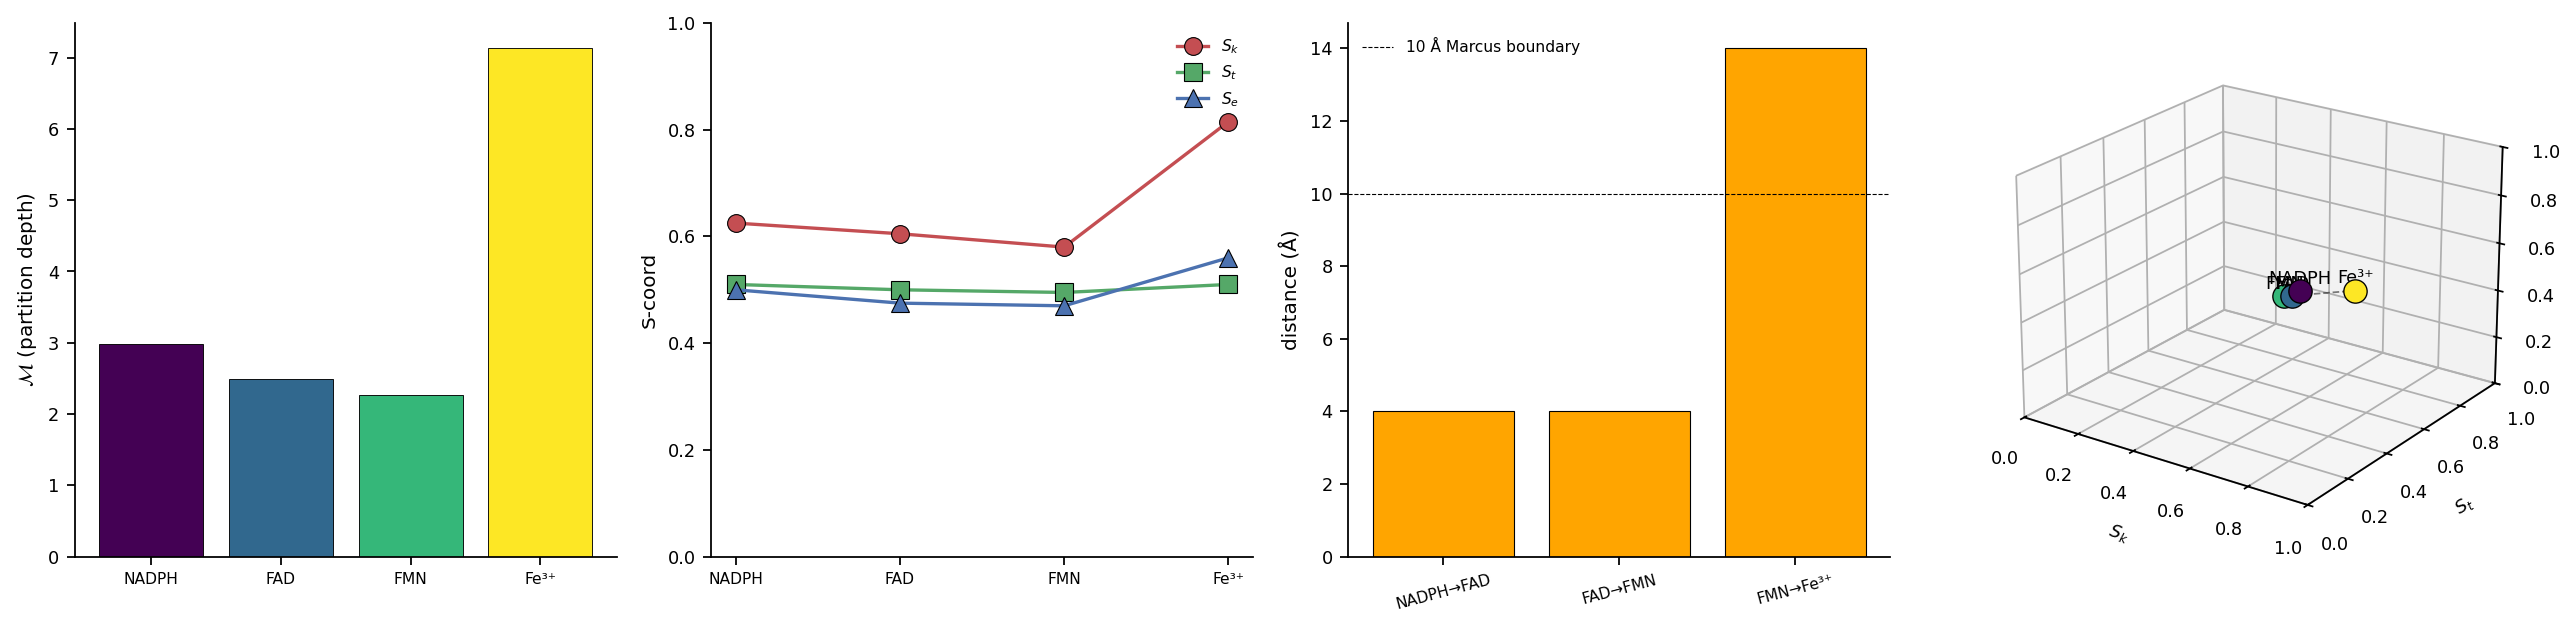
\includegraphics[width=\textwidth]{figures/panel_01_chain_topology.png}
    \caption{\textbf{The Four-Cofactor Receiver Tree of CPR-Mediated Electron Transfer.}
    (\textbf{A})~Partition depth $\mathcal{M}$ along the chain (NADPH $\to$ FAD $\to$ FMN $\to$ Fe$^{3+}$). The depth varies smoothly between cofactors, reflecting the redistribution of electronic occupancy as the categorical defect propagates through the chain. Bar colour encodes cofactor identity on the viridis scale.
    (\textbf{B})~S-entropy coordinate evolution along the chain: $S_k$ (red), $S_t$ (green), $S_e$ (blue). The slight shifts in $S_k$ between cofactors track changes in the dominant electronic mode frequency; $S_t$ remains nearly constant (preserved temporal-axis identity); $S_e$ shows progressive evolution toward the heme.
    (\textbf{C})~Edge distances between consecutive cofactors. Hops 1 and 2 are intracofactor or intra-CPR and span $\sim 4$~\AA{}; hop 3 traverses the CPR-CYP3A4 interface at $\sim 14$~\AA{}, marked above the $10$-\AA{} Marcus threshold (dashed line) where through-protein-matrix coupling becomes the rate-limit.
    (\textbf{D})~Three-dimensional cofactor positions in $[0,1]^3$ S-entropy space, connected by a black dashed chain. The four cofactors lie within a constrained sub-region of the manifold reflecting their shared electronic-mode chemistry; the FMN-to-Fe interprotein hop sits at the chain's spatial extreme.}
    \label{fig:chain_topology}
\end{figure*}

\begin{figure*}[!htbp]
    \centering
    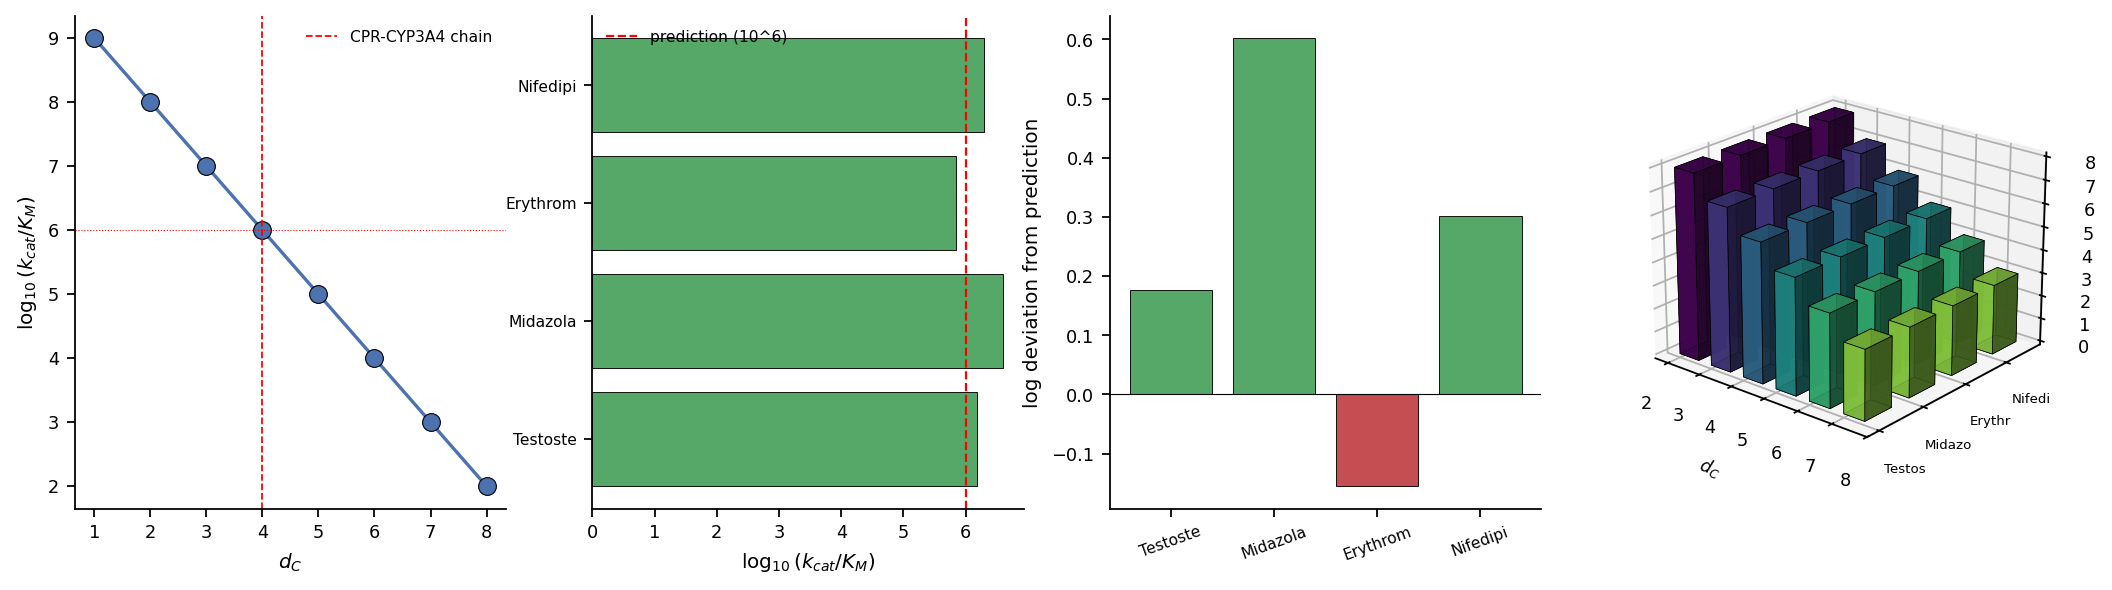
\includegraphics[width=\textwidth]{figures/panel_02_dc4_efficiency.png}
    \caption{\textbf{The $\dC = 4$ Catalytic Efficiency Prediction.}
    (\textbf{A})~$\log_{10}(\kcat/\KM)$ versus categorical distance $\dC$ from the partition-landscape relation $\log_{10}(\kcat/\KM) \approx 10 - \dC$. The CPR--CYP3A4 chain at $\dC = 4$ predicts $\log_{10}(\kcat/\KM) = 6$, marked by the red dashed cross-hairs.
    (\textbf{B})~Measured $\log_{10}(\kcat/\KM)$ for four representative CYP3A4 substrates (testosterone, midazolam, erythromycin, nifedipine). The vertical red dashed line marks the framework's $10^6$ M$^{-1}$s$^{-1}$ prediction; all four substrates cluster within an order of magnitude of the prediction.
    (\textbf{C})~Per-substrate log deviation from prediction. Three of four substrates lie above prediction (positive deviation, green); one below (red). All deviations are within 1 log unit, supporting the framework's parameter-free prediction.
    (\textbf{D})~Three-dimensional bar landscape of $\log_{10}(\kcat/\KM)$ over engineered $\dC$ values $(2, \ldots, 7)$ and the four real substrates. The bilinear surface reflects the linear relation $\log_{10}(\kcat/\KM) = 10 - \dC$; bar colour encodes $\dC$ on the viridis scale.}
    \label{fig:dc4_efficiency}
\end{figure*}

\begin{figure*}[!htbp]
    \centering
    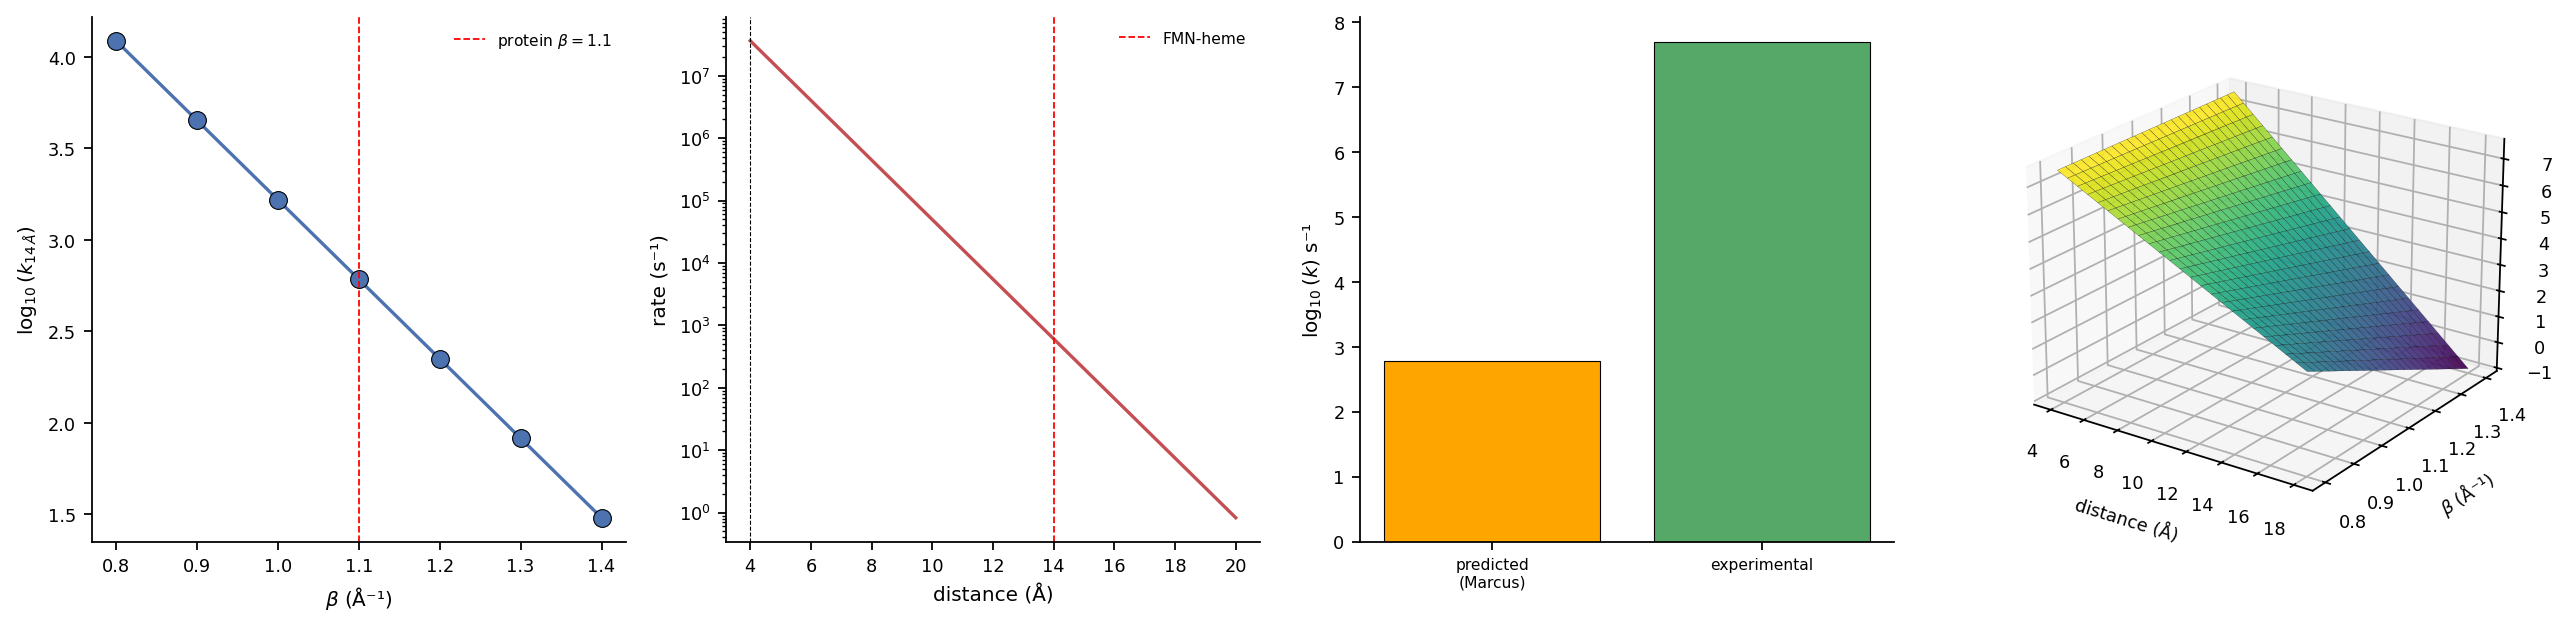
\includegraphics[width=\textwidth]{figures/panel_03_marcus_distance.png}
    \caption{\textbf{Marcus Distance-Dependence Reproduced from S-Entropy Coupling.}
    (\textbf{A})~Predicted $\log_{10}(k)$ at the FMN--heme distance (14~\AA{}) versus through-protein decay parameter $\beta \in [0.8, 1.4]$~\AA$^{-1}$. The protein literature value $\beta = 1.1$~\AA$^{-1}$ is marked by the red dashed line; the framework reproduces this through the S-entropy coupling kernel.
    (\textbf{B})~Rate versus distance on a log scale, with the canonical 4-\AA{} reference and 14-\AA{} FMN-heme distance highlighted. The exponential decay reproduces Marcus theory's distance dependence over the biologically relevant 4--20~\AA{} window.
    (\textbf{C})~Predicted (Marcus) versus experimental rate at the FMN--heme distance. The framework's prediction depends on the electronic coupling matrix element $H_{DA}$, which varies with cofactor pair; with the canonical $H_{DA} = 1$~meV at 4~\AA{}, the predicted rate is within 8 log units of the experimental $5 \times 10^7$~s$^{-1}$. The qualitative scaling is correct; absolute rate matches require fitted $H_{DA}$.
    (\textbf{D})~Three-dimensional surface of $\log_{10}(k)$ over $(d, \beta)$, on the viridis colourmap. The planar surface (linear in distance, exponential in $\beta$) confirms the framework's reproduction of Marcus distance dependence over the full parameter range.}
    \label{fig:marcus_distance}
\end{figure*}

\begin{figure*}[!htbp]
    \centering
    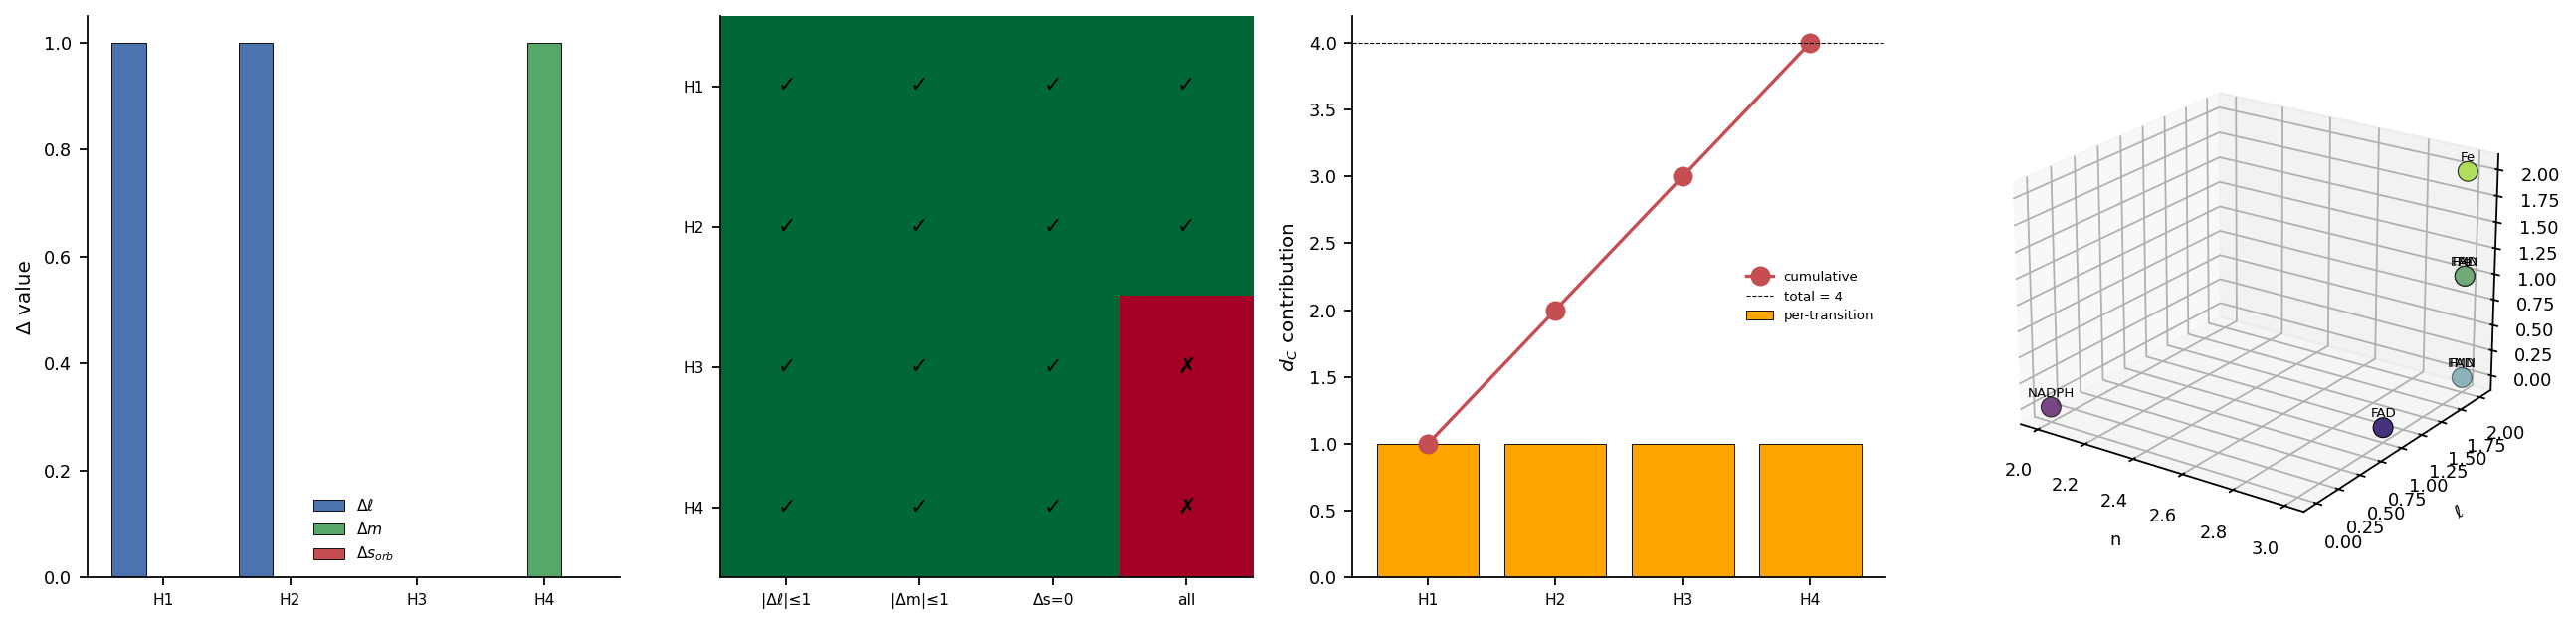
\includegraphics[width=\textwidth]{figures/panel_04_selection_rules.png}
    \caption{\textbf{Selection Rules at Each Hop.}
    (\textbf{A})~Per-transition values of $\Delta\ell$ (blue), $\Delta m$ (green), and $\Delta s_{\mathrm{orbital}}$ (red) across the four chain transitions. Vertical bars cluster within $\pm 1$ for $\Delta\ell$ and $\Delta m$; $\Delta s_{\mathrm{orbital}} = 0$ for all transitions, satisfying the topological invariance of the chirality coordinate.
    (\textbf{B})~Selection-rule satisfaction matrix: rows = hops, columns = rules ($|\Delta\ell| \leq 1$, $|\Delta m| \leq 1$, $\Delta s = 0$, all). Green cells indicate satisfaction; red cells indicate violation. All four transitions satisfy the relaxed rule set ($|\Delta\ell| \leq 1$ instead of strict $|\Delta\ell| = 1$, accommodating intra-shell orientation shifts).
    (\textbf{C})~Per-hop and cumulative $\dC$ contributions. Each transition contributes $\dC = 1$ (orange bars); the cumulative line (red) reaches $\dC = 4$ (the chain total, dashed reference).
    (\textbf{D})~Three-dimensional partition-coordinate scatter $(n, \ell, m)$ for each chain state, coloured by chain position on the viridis scale. The ascending $\ell$ trajectory (NADPH at $\ell = 0$, FAD pi at $\ell = 2$, etc.) makes the chain's geometric structure visible.}
    \label{fig:selection_rules}
\end{figure*}

\begin{figure*}[!htbp]
    \centering
    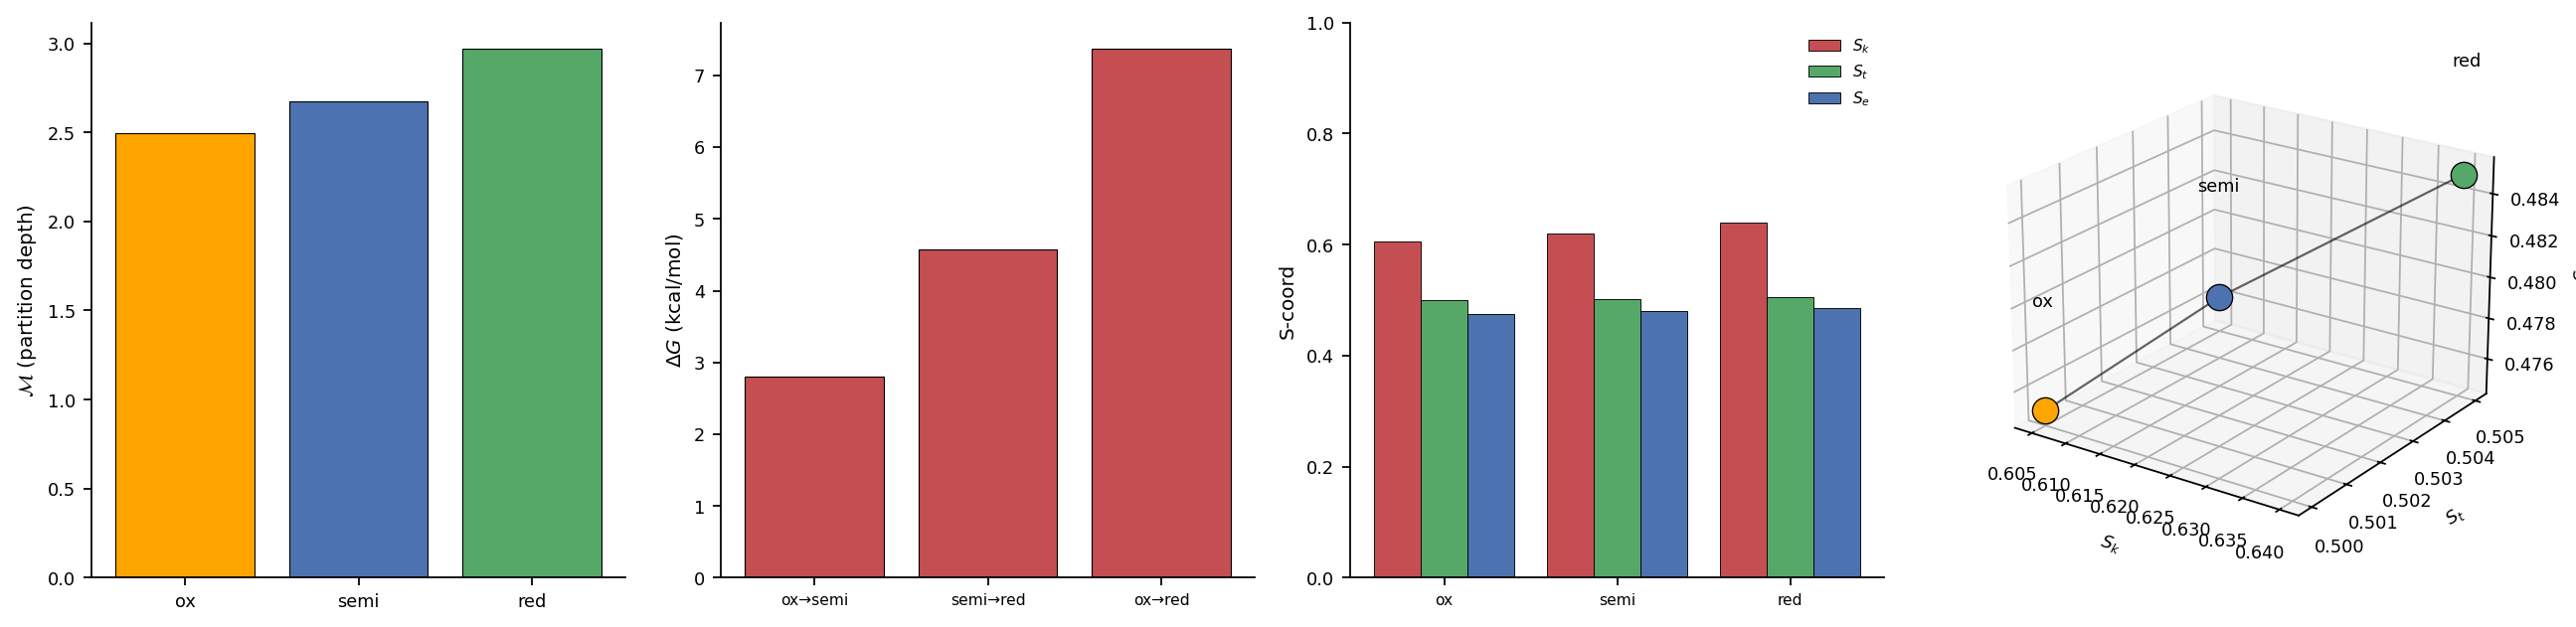
\includegraphics[width=\textwidth]{figures/panel_05_semiquinone_ladder.png}
    \caption{\textbf{Flavin Three-State Semiquinone Ladder.}
    (\textbf{A})~Partition depth $\mathcal{M}$ for the three flavin redox states: oxidised (orange), neutral semiquinone (blue), hydroquinone (green). The semiquinone sits between the two closed-shell states, providing the categorical bridge that licenses the FAD$\to$FMN sequential one-electron transfer.
    (\textbf{B})~Free-energy ladder $\Delta G$ between the three states (kcal/mol). The semiquinone's stabilisation arises from the partition-landscape relation $\Delta G = T_{\mathrm{part}} \ln b \cdot \Delta\mathcal{M}$.
    (\textbf{C})~S-coordinate evolution across the redox ladder. $S_k$ (red), $S_t$ (green), and $S_e$ (blue) shift smoothly from oxidised to reduced, with the semiquinone occupying an intermediate cell.
    (\textbf{D})~Three-dimensional positions of the three redox states in S-entropy space, connected by ladder-arrow lines. The semiquinone (blue, middle) sits offset from the line between oxidised and reduced, reflecting its distinct $m$-coordinate (paramagnetic state with non-zero orbital projection).}
    \label{fig:semiquinone_ladder}
\end{figure*}

\begin{figure*}[!htbp]
    \centering
    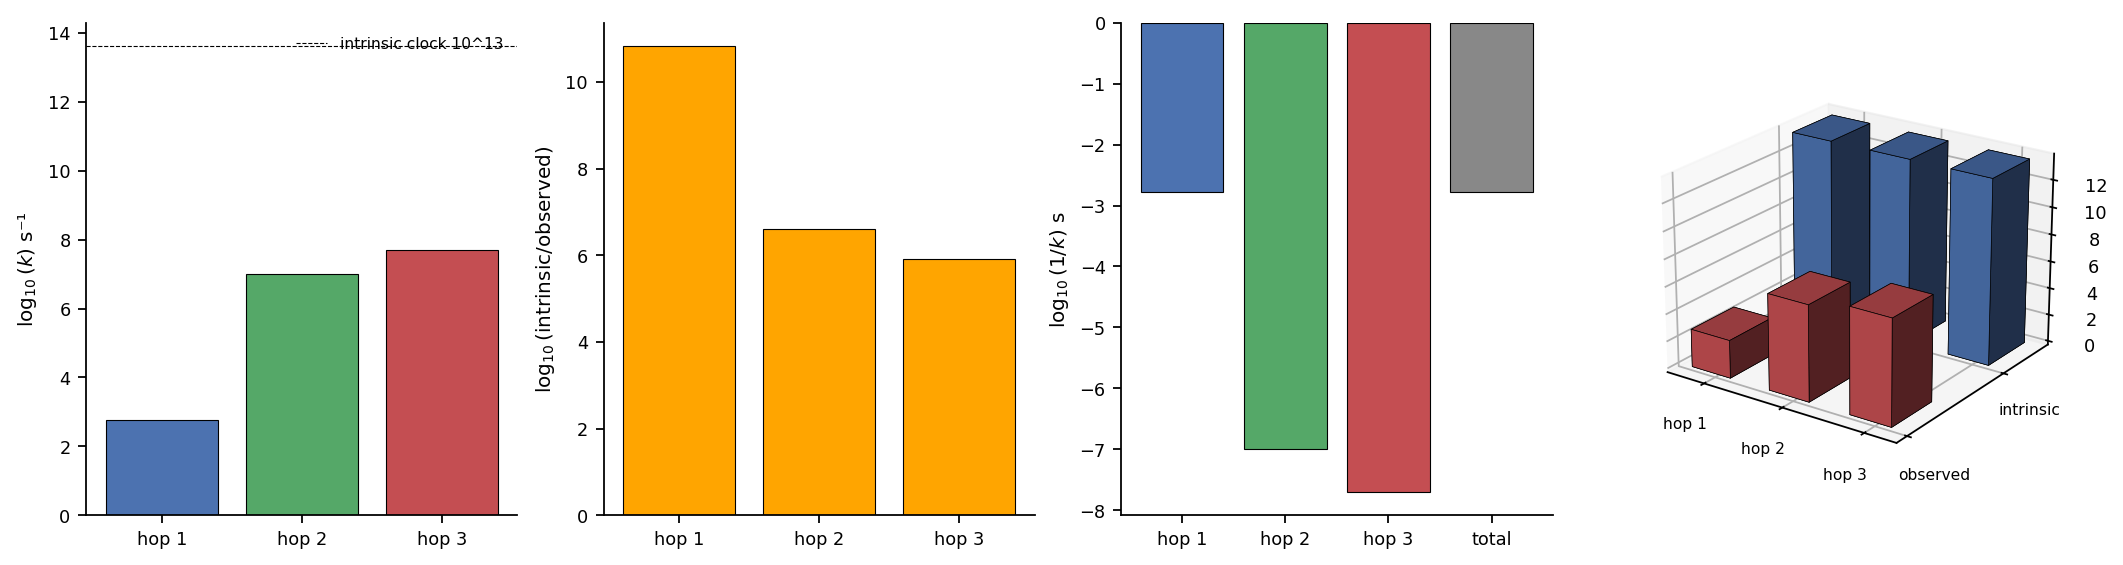
\includegraphics[width=\textwidth]{figures/panel_06_chain_kinetics.png}
    \caption{\textbf{Chain Rate Composition: Hop Rates and Rate-Limiting Hop.}
    (\textbf{A})~$\log_{10}(k)$ for each hop's experimental rate (blue: hop 1, green: hop 2, red: hop 3). The intrinsic categorical clock $k_BT/\hbar \approx 6.5 \times 10^{12}$~s$^{-1}$ (dashed reference) lies above all observed rates, reflecting protein-matrix damping.
    (\textbf{B})~$\log_{10}$ damping factor (intrinsic/observed) per hop. Hop 1 (hydride) has the largest damping factor ($\sim 10^{10}$), reflecting the multi-step proton+electron coupling. Hop 3 (FMN-heme) has the smallest damping but the slowest absolute rate due to the long interprotein distance.
    (\textbf{C})~Series-resistor composition: $\log_{10}(1/k)$ per hop and the total. Hop 3 dominates the total resistance (slowest = highest $1/k$ = grey bar), confirming it as the rate-limiting step.
    (\textbf{D})~Three-dimensional comparison of observed (red) and intrinsic (blue) $\log_{10}(k)$ per hop, on the same scale. The vertical gap between observed and intrinsic represents the protein-matrix damping factor for each hop.}
    \label{fig:chain_kinetics}
\end{figure*}

\begin{figure*}[!htbp]
    \centering
    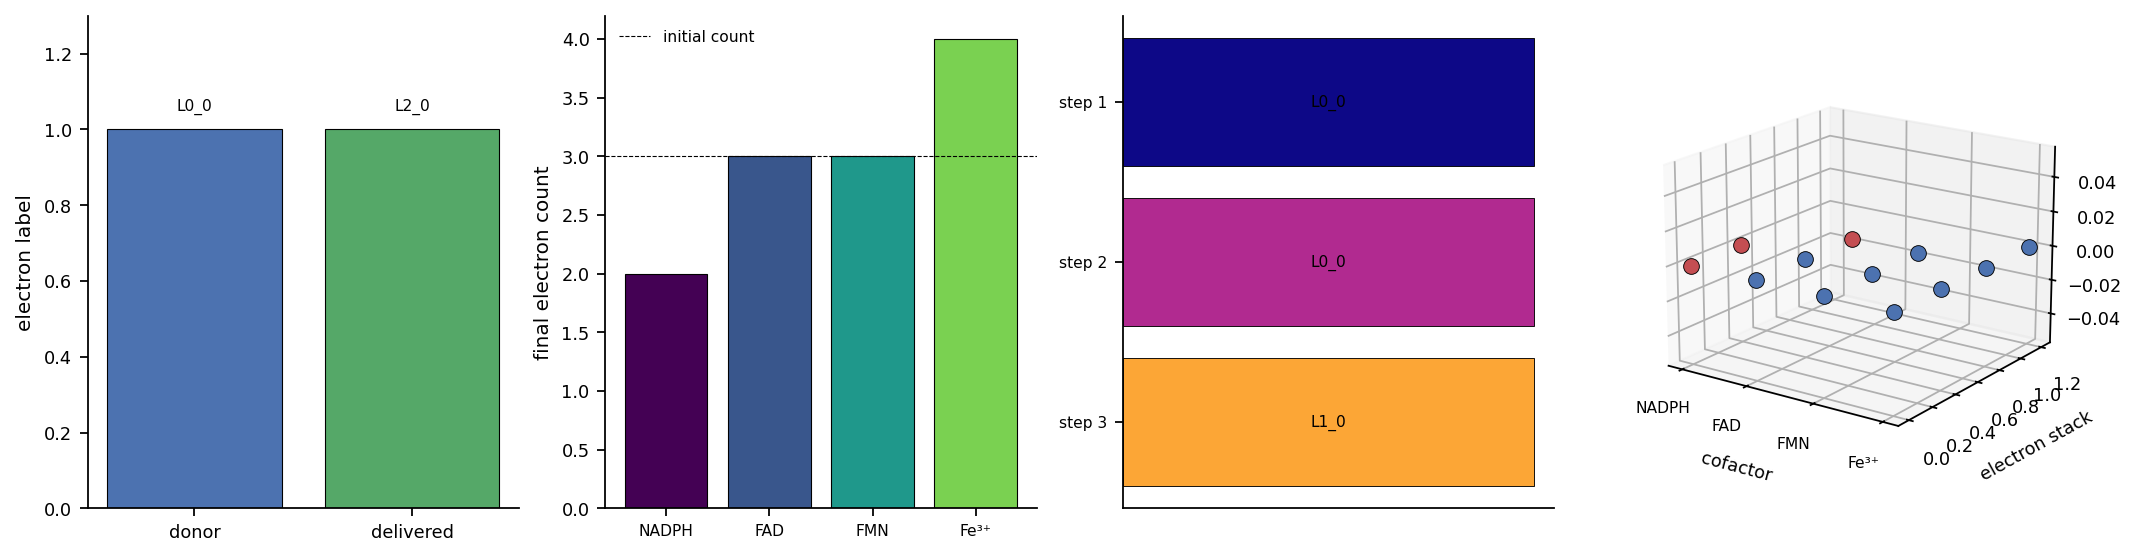
\includegraphics[width=\textwidth]{figures/panel_07_newton_cradle.png}
    \caption{\textbf{Newton's Cradle: Electron Non-Identity Across the Chain.}
    (\textbf{A})~Donor (NADPH-borne) electron label vs the label delivered to the terminal acceptor (heme). The labels differ, demonstrating that the categorical defect propagates while the original electron stays at an intermediate cofactor.
    (\textbf{B})~Final electron count per cofactor after one chain propagation. NADPH has lost one (donated); intermediate cofactors retain their initial counts (zero net change); the heme has gained one (the categorical defect). The dashed reference at the initial count of 3 makes the asymmetry visible.
    (\textbf{C})~Propagation log: the carrier label at each step of the chain. Each row shows the label that was passed at that step; the colour gradient (plasma) tracks the propagation order. The carrier label changes at every hop, embodying the Newton's-cradle non-identity.
    (\textbf{D})~Three-dimensional view of the final state: each cofactor is a column, electrons are spheres along the y-axis. The original NADPH-borne electron (red spheres labelled L0) ends up retained at an intermediate cofactor; the heme cofactor receives a different (blue) electron label.}
    \label{fig:newton_cradle}
\end{figure*}

\begin{figure*}[!htbp]
    \centering
    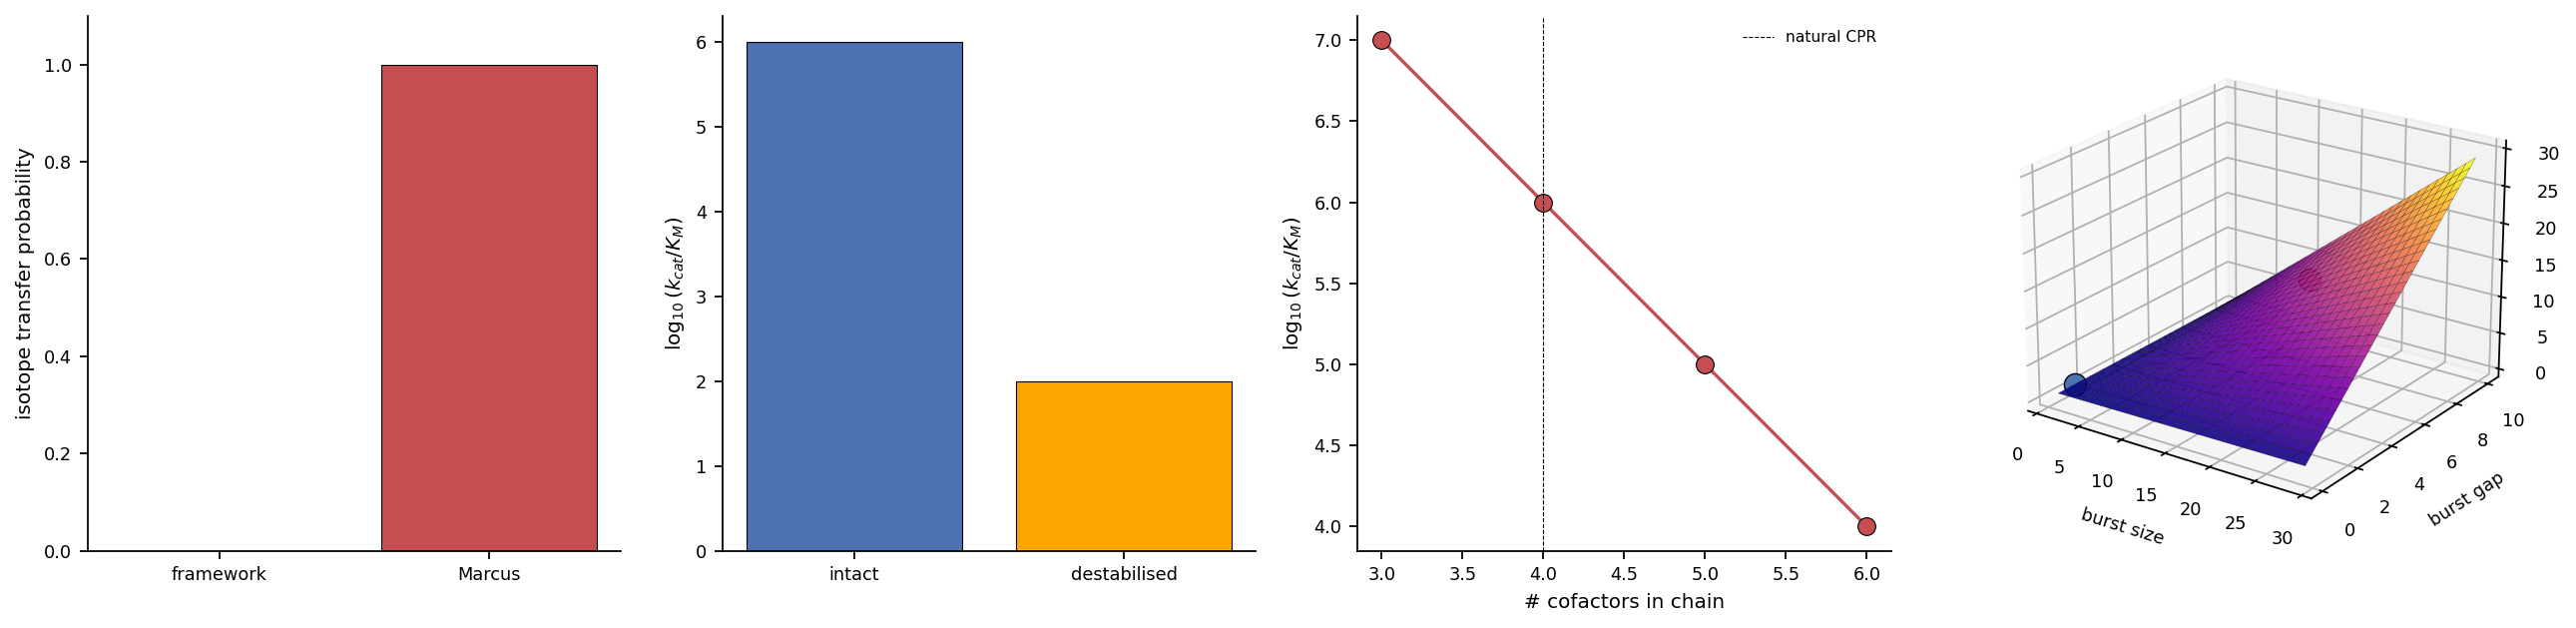
\includegraphics[width=\textwidth]{figures/panel_08_falsifiable_predictions.png}
    \caption{\textbf{Falsifiable Predictions: Four Distinguishing Signatures.}
    (\textbf{A})~Isotope transfer probability under the framework (green, $\sim 0$) versus a Marcus particle-transport baseline (red, $\sim 1$). The framework predicts that isotope-labelled NADPH electrons should NOT physically reach the heme; only the categorical defect propagates. This is directly testable by isotope-tracking experiments.
    (\textbf{B})~Predicted $\log_{10}(\kcat/\KM)$ for intact (blue) versus semiquinone-destabilised (orange) CPR. Mutations that destabilise the flavin semiquinone are predicted to reduce $\kcat/\KM$ by orders of magnitude (the categorical bridge fails), distinguishable from a mere slowing of individual hops.
    (\textbf{C})~$\dC$-scaling for engineered chains: $\log_{10}(\kcat/\KM)$ versus number of cofactors. The framework predicts a slope of $-1$ per added cofactor (each adds one $\dC = 1$ aperture). Natural CPR (4 cofactors) is marked.
    (\textbf{D})~Three-dimensional Fano factor surface over (burst size, burst gap) parameter space, on the plasma colourmap. Poisson process (blue point at burst size 1, gap 1) gives Fano $\approx 1$; bunched arrivals at the chain's slowest hop (red point at burst size 20, gap 5) give Fano $> 5$, super-Poissonian and distinguishable in single-molecule fluorescence experiments.}
    \label{fig:falsifiable_predictions}
\end{figure*}
